En este capítulo se establecen los fundamentos teóricos y prácticos del trabajo. Se inicia con una introducción al modelado de sistemas y los principios del aprendizaje automático supervisado, utilizando la regresión lineal y logística como ejemplos introductorios y detallando el método de optimización por descenso de gradiente. A continuación, se presentan las métricas de evaluación para tareas de regresión y clasificación. Posteriormente, se profundiza en las redes neuronales, desde el perceptrón simple hasta el perceptrón multicapa (MLP), explicando en detalle el algoritmo de entrenamiento por retropropagación (\textit{backpropagation}). Luego, se introduce el concepto de compresión, enfocándose en las técnicas aplicadas a redes neuronales, para finalmente centrarse en la cuantización. Se describen sus tipos y las dos estrategias principales: la cuantización post-entrenamiento (PTQ) y la cuantización consciente del entrenamiento (QAT). Se explica el mecanismo de QAT, destacando el problema de los gradientes en funciones no diferenciables y el rol del estimador \textit{Straight-Through Estimator} (STE) como solución. Finalmente, se presentan los \textit{frameworks} de software utilizados, \texttt{TensorFlow} y \texttt{TensorFlow Model Optimization}, y la funcionalidad de los gradientes personalizados, una herramienta clave para la implementación del STE.

\section{Modelado de sistemas}
\label{sec:modelado_de_sistemas}

El modelado de sistemas y de relaciones entre variables es una tarea fundamental en múltiples áreas de la ingeniería y la ciencia. Un sistema puede definirse como una relación funcional entre variables de entrada $x$ y salida $y$, donde la salida es una función de las entradas $y = f(x)$, como se muestra en la \reffig{system}.

\begin{figure}[H]
    \centering
    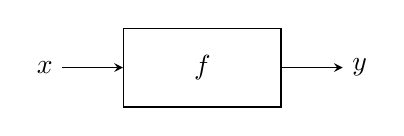
\begin{tikzpicture}
        \node (input) at (0, 0) [] {$x$};
        \node (output) at (4, 0) [] {$y$};
        \node[rectangle,, draw, minimum width=2cm, minimum height=1cm] (system) at (2, 0) {$f$};
        \draw[-stealth] (input) -- (system);
        \draw[-stealth] (system) -- (output);
    \end{tikzpicture}
    \caption{Sistema a modelar.}
    \label{fig:system}
\end{figure}

En este contexto, se busca aproximar la relación $y = f(x)$ mediante un modelo $\hat{f}$, con parámetros $\theta$, que permita estimar la salida $\hat{y}$ a partir de la entrada $x$, como se muestra en la \refeq{system_approximation} y la \reffig{system_model}.

\begin{equation}
    \label{eq:system_approximation}
    \hat{y} = \hat{f}(x; \theta) \approx f(x)
\end{equation}

\begin{figure}[H]
    \centering
    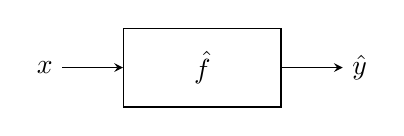
\begin{tikzpicture}
        \node (input) at (0, 0) [] {$x$};
        \node (output) at (4, 0) [] {$\hat{y}$};
        \node[rectangle,, draw, minimum width=2cm, minimum height=1cm] (system) at (2, 0) {$\hat{f}$};
        \draw[-stealth] (input) -- (system);
        \draw[-stealth] (system) -- (output);
    \end{tikzpicture}
    \caption{Modelo del sistema.}
    \label{fig:system_model}
\end{figure}

Con este objetivo, se define un problema de optimización a partir de una función de costo $L$ que mide el error entre la salida real $y$ y la salida estimada $\hat{y}$. A continuación, se buscan los parámetros $\theta$ que minimicen la función de costo $L(y, \hat{y})$. Generalmente, la función de costo incluye términos adicionales independientes del error, por ejemplo, penalizaciones para desalentar comportamientos no deseados del modelo \cite{Ng2004}.

En cuanto al tipo de salida, se distinguen dos clases de problemas de modelado: regresión y clasificación. La diferencia radica en el espacio de salida $y$. En los problemas de regresión, la variable de salida es continua, mientras que en los problemas de clasificación, la variable de salida es discreta y representa categorías o clases. Además de las funciones de costo, es importante seleccionar métricas de evaluación adecuadas para cada tipo de problema, que permitan cuantificar el desempeño del modelo en función de los objetivos específicos del mismo; dichas métricas se detallan en la sección \ref{sec:metricas}.

El proceso de encontrar los parámetros óptimos $\theta$ se denomina entrenamiento. Existen casos en los que se dispone de soluciones cerradas que pueden calcularse analíticamente. Sin embargo, en la mayoría de los problemas se emplean métodos numéricos iterativos para aproximar la solución óptima, dado que las soluciones cerradas son poco frecuentes en aplicaciones reales \cite{e23081012}.

Para llevar a cabo este proceso de entrenamiento, se requiere un conjunto de datos de entrada y salida conocidos (etiquetados) $\left(x_i, y_i\right)$, denominado conjunto de entrenamiento (o \textit{dataset} en inglés). Este tipo de aprendizaje se denomina aprendizaje supervisado, ya que estima una función a partir de datos etiquetados.

\subsection{Gradiente descendiente}
\label{sec:gradiente_descendiente}

El método iterativo más utilizado para ajustar los parámetros es el descenso por gradiente, que consiste en actualizar los parámetros en la dirección contraria al gradiente de la función de costo ($\nabla_{\theta} L(y, \hat{y})$), es decir, en la dirección que reduce el error \cite{9603742}. La actualización de los parámetros se realiza como se muestra en la ecuación \ref{eq:gradient_descent}, donde $\eta$ es la tasa de aprendizaje, que determina el tamaño del paso en cada iteración.

\begin{equation}
    \label{eq:gradient_descent}
    \theta_{n+1} = \theta_n - \eta \nabla_{\theta} L(y, \hat{y})
\end{equation}

Una variante de este algoritmo es el descenso por gradiente estocástico (de ahora en adelante SGD, por sus siglas en inglés de \textit{Stochastic Gradient Descent}), que utiliza un subconjunto aleatorio de los datos de entrenamiento en cada iteración para calcular el gradiente; véase la \refeq{sgd}. Esto reduce el costo computacional y puede ayudar a escapar de mínimos locales. Aunque introduce más ruido en el proceso de optimización, puede acelerar la convergencia \cite{robbins1951stochastic}.

\begin{equation}
    \label{eq:sgd}
    \theta_{n+1} = \theta_n - \eta \nabla_{\theta} L(y_i, \hat{y}_i)
\end{equation}

\subsection{Regresión lineal}
\label{sec:regresion_lineal}
El modelo de regresión lineal es uno de los modelos más simples y ampliamente utilizados en el aprendizaje supervisado \cite{Hastie2009}. Este modelo provee una estimación de una variable continua $y$ a partir de una variable independiente $x$, cuya relación se modela con una recta, como se muestra en la \refeq{linear_regression}.

\begin{equation}
    \label{eq:linear_regression}
    \hat{y} = \theta_0 + \theta_1 x
\end{equation}

Para ello, el objetivo es ajustar los parámetros $\theta_0$, $\theta_1$ que minimicen alguna métrica de error, definida por una función de costo $L$. En el caso de la regresión lineal, la función de costo utilizada comúnmente es el error cuadrático medio (o MSE por sus siglas en inglés \textit{Mean Squared Error}). Además, si se extrapola este modelo a un problema multivariable, la \refeq{linear_regression} se puede expresar como se muestra en la \refeq{linear_regression_multivariable}.

\begin{equation}
    \label{eq:linear_regression_multivariable}
    \hat{y} = \theta_0 + \sum_{j=1}^{m} \theta_j x_j
\end{equation}

En consecuencia, se buscan los valores de $\theta_0$, $\theta_1$, ..., $\theta_m$ que minimicen la función de costo definida en la \refeq{mse}. Para ello, se utiliza un conjunto de datos de tamaño $n$, donde $\mathbf{y}$ es el vector de salidas reales y $\hat{\mathbf{y}}$ es el vector de salidas estimadas por el modelo para las entradas correspondientes $\mathbf{X}$.

\begin{equation}
    \label{eq:mse}
    L(\mathbf{y}, \hat{\mathbf{y}}) = \frac{1}{n} \sum_{i=1}^{n} \left(y_i - \hat{y}_i\right)^2
\end{equation}

Para este problema particular, es posible deducir analíticamente los valores de $\mathbf{\theta}$ que minimizan la función de costo. Para esto, se deriva la función de costo con respecto a los parámetros $\frac{\partial L(\mathbf{y}, \hat{\mathbf{y}})}{\partial \mathbf{\theta}}$ y se iguala a cero. Al realizar esto, se obtiene la fórmula conocida como OLS (por sus siglas en inglés \textit{Ordinary Least Squares}), que permite calcular los parámetros óptimos de manera directa, como se muestra en la \refeq{ols}, donde $\mathbf{X}$ es la matriz de características, $\mathbf{\theta}$ es el vector de parámetros, y $\mathbf{y}$ es el vector de salidas reales, como se muestra en la \refeq{ols_matrices}.

\begin{equation}
    \label{eq:ols}
        \theta = \left(X^T X\right)^{-1} X^T y
\end{equation}

\begin{equation}
    \label{eq:ols_matrices}
      X =
        \begin{bmatrix}
        1 & x_{1,1} & x_{2,1} & \dots & x_{n,1} \\
        1 & x_{1,2} & x_{2,2} & \dots & x_{n,2} \\
        \vdots & \vdots & \vdots & \dots & \vdots \\
        1 & x_{1,m} & x_{2,m} & \dots & x_{n,m}
        \end{bmatrix}
      \quad \quad
      \theta =
        \begin{bmatrix}
          \theta_0 \\ \theta_1 \\ \theta_2 \\ \dots \\ \theta_n
        \end{bmatrix}
      \quad \quad
      y = \begin{bmatrix} y_1 \\ y_2 \\ \vdots \\ y_m \end{bmatrix}
    \end{equation}


Por lo tanto, este es un caso con solución cerrada, ya que permite calcular los parámetros óptimos de manera directa sin necesidad de utilizar métodos iterativos como el descenso por gradiente.

A modo de ilustración, el resultado de aplicar este modelo a un conjunto de datos se muestra en la \reffig{linear_regression}, donde se observa la línea de regresión ajustada a los datos, así como los errores entre las predicciones del modelo y los datos reales.

\defaultfigurecustomsize{regression/linear_regression.png}{Regresión Lineal.}{linear_regression}{1.1}

\subsection{Regresión logística}
\label{sec:regresion_logistica}

El modelo de regresión logística se utiliza en problemas de clasificación binaria. Estima la probabilidad de que una observación pertenezca a una clase mediante la función sigmoide \cite{Hosmer2013}, como se muestra en la \refeq{logistic_regression}.

\begin{equation}
    \label{eq:logistic_regression}
    \hat{y} = \mathbb{P}\left(y=1 \mid x\right)  = \frac{1}{1 + e^{-\left(\theta_0 + \sum_{j=1}^{m} \theta_j x_j\right)}}
\end{equation}

El valor de salida $\hat{y}$ pertenece al intervalo $(0, 1)$ y representa la probabilidad de que la observación pertenezca a la clase 1. En la práctica, se utiliza un umbral (comúnmente $0.5$). Si $\hat{y} \geq 0.5$, la observación se asigna a la clase 1; en caso contrario, a la clase 0. Véase la \reffig{logistic_regression}.

\defaultfigurecustomsize{regression/logistic_regression.png}{Regresión Logística.}{logistic_regression}{1.1}

En este modelo, la función de costo se define a partir de la verosimilitud. Bajo la hipótesis de independencia de las observaciones, la verosimilitud mide cuán probable resulta observar los datos dados los parámetros del modelo y se expresa como en la \refeq{likelihood} para una muestra de tamaño $n$.

\begin{equation}
    \label{eq:likelihood}
      V(\theta) = \prod_{i=1}^{n} \mathbb{P}(y_i \mid x_i)
\end{equation}

donde $\mathbb{P}(y_i \mid x_i)$ es la probabilidad de observar la clase $y_i$ dado el vector de características $x_i$. Por conveniencia computacional, se trabaja con el logaritmo de la función de verosimilitud, conocido como log-verosimilitud, que convierte el producto en una suma, como se muestra en la \refeq{log_likelihood}.

\begin{equation}
    \label{eq:log_likelihood}
      \ell(\theta) = \sum_{i=1}^{n} \left[ y_i \log(\mathbb{P}(y_i \mid x_i)) + (1 - y_i) \log(1 - \mathbb{P}(y_i \mid x_i)) \right]
\end{equation}

En consecuencia, la función de costo se define como el negativo de la log-verosimilitud; por lo tanto, el problema se plantea como la minimización de dicha función (equivalente a maximizar la log-verosimilitud) con respecto a los parámetros $\theta$. Dado que no existe una solución cerrada para este problema, se emplean métodos numéricos iterativos; en particular, el descenso por gradiente permite aproximar los parámetros que maximizan la verosimilitud.

\TODO{Revisar esta ultima parte}
En el caso de problemas con clasificación multiclase, se suele utilizar la función de costo de entropía cruzada generalizada (\textit{categorical cross-entropy} en inglés) cuya ecuación se muestra en la \refeq{categorical_cross_entropy} y la función de activación \textit{softmax}, cuya ecuación se muestra en la \refeq{softmax}, para modelar las probabilidades de pertenencia a cada clase.

\begin{equation}
    \label{eq:categorical_cross_entropy}
    L(\mathbf{y}, \hat{\mathbf{y}}) = - \sum_{i=1}^{n} \sum_{c=1}^{C} y_{i,c} \log(\hat{y}_{i,c})
\end{equation}

\begin{equation}
    \label{eq:softmax}
    \hat{y}_{i,c} = \frac{e^{z_{i,c}}}{\sum_{k=1}^{C} e^{z_{i,k}}}
\end{equation}

donde $C$ es el número de clases, $y_{i,c}$ es una variable indicadora que vale 1 si la observación $i$ pertenece a la clase $c$ y 0 en caso contrario, e $\hat{y}_{i,c}$ es la probabilidad estimada de que la observación $i$ pertenezca a la clase $c$, calculada mediante la función \textit{softmax} aplicada a los logits $z_{i,c}$.

\section{Métricas de evaluación}
\label{sec:metricas}

En el contexto de modelos de \textit{machine learning}, las métricas de evaluación son herramientas fundamentales para cuantificar el desempeño de un modelo en tareas específicas. Estas métricas permiten comparar diferentes modelos, ajustar hiperparámetros y validar la efectividad del aprendizaje. La elección de la métrica adecuada depende del tipo de problema que se esté abordando.


\subsection{Métricas para problemas de regresión}
\label{sec:metricas_regresion}

Algunas métricas comunes para problemas de regresión son:

\begin{itemize}
    \item Error cuadrático medio (MSE, por sus siglas del inglés \textit{Mean Squared Error}): Calcula la media de los cuadrados de las diferencias entre las predicciones y los valores reales. \cite{botchkarev2019performance}
    \begin{equation}
        \text{MSE} = \frac{1}{n} \sum_{i=1}^{n} (y_i - \hat{y}_i)^2
    \end{equation}

    \item Error absoluto medio (MAE, por sus siglas del inglés \textit{Mean Absolute Error}): Calcula la media de las diferencias absolutas entre las predicciones y los valores reales. \cite{willmott2005advantages}
    \begin{equation}
        \text{MAE} = \frac{1}{n} \sum_{i=1}^{n} |y_i - \hat{y}_i|
    \end{equation}

    \item Coeficiente de determinación ($R^2$): Mide la proporción de la varianza en los datos que es explicada por el modelo. Un valor de $R^2$ cercano a 1 indica un buen ajuste. \cite{alexander2016rsquared}
    \begin{equation}
        R^2 = 1 - \frac{\sum_{i=1}^{n} (y_i - \hat{y}_i)^2}{\sum_{i=1}^{n} (y_i - \bar{y})^2}
    \end{equation}
\end{itemize}

\subsection{Métricas para problemas de clasificación}
\label{sec:metricas_clasificacion}
Para el caso de los problemas de clasificación, se suelen utilizar métricas definidas a partir de los siguientes conceptos: \textit{verdaderos positivos} (TP, por sus siglas del inglés \textit{True Positives}), que corresponden al número de instancias positivas correctamente clasificadas como positivas; \textit{falsos positivos} (FP, por sus siglas del inglés \textit{False Positives}), que representan el número de instancias negativas incorrectamente clasificadas como positivas; \textit{verdaderos negativos} (TN, por sus siglas del inglés \textit{True Negatives}), que son el número de instancias negativas correctamente clasificadas como negativas; y \textit{falsos negativos} (FN, por sus siglas del inglés \textit{False Negatives}), que indican el número de instancias positivas incorrectamente clasificadas como negativas. En la \ref{tab:confusion_matrix} se muestra una matriz de confusión \cite{sokolova2009systematic} que resume estos conceptos para un problema de clasificación binaria.

\begin{table}[H]
    \centering
    \caption{Matriz de confusión para un problema de clasificación binaria.}
    \begin{tabular}{c c c}
        \toprule
        & \textbf{Predicción Positiva} & \textbf{Predicción Negativa} \\
        \midrule
        \textbf{Clase Positiva} & TP & FN \\
        \textbf{Clase Negativa} & FP & TN \\
        \bottomrule
        \hline
    \end{tabular}
    \label{tab:confusion_matrix}
\end{table}

\begin{itemize}
    \item Exactitud (\textit{accuracy} en inglés): Mide la proporción de predicciones correctas sobre el total de predicciones. Se computa como se muestra en la \refeq{accuracy} \cite{bishop2006pattern}.
    \begin{equation}
        \label{eq:accuracy}
        \text{accuracy} = \frac{TP + TN}{TP + TN + FP + FN}
    \end{equation}
    \item Precisión (\textit{precision} en inglés): Mide la proporción de predicciones positivas correctas sobre el total de predicciones positivas. Se computa como se muestra en la \refeq{precision} \cite{bishop2006pattern}.
    \begin{equation}
        \label{eq:precision}
        \text{precision} = \frac{TP}{TP + FP}
    \end{equation}
    \item Sensibilidad (\textit{recall} en inglés): Mide la proporción de verdaderos positivos sobre el total de positivos reales. Se computa como se muestra en la \refeq{recall} \cite{bishop2006pattern}.
    \begin{equation}
        \label{eq:recall}
        \text{recall} = \frac{TP}{TP + FN}
    \end{equation}
    \item Puntaje F1 (\textit{F1-score} en inglés): Es la media armónica entre la precisión y la sensibilidad, proporcionando un balance entre ambas métricas. Se computa como se muestra en la \refeq{f1_score} \cite{bishop2006pattern}.
    \begin{equation}
        \label{eq:f1_score}
        \text{F1-score} = 2 \cdot \frac{\text{precision} \cdot \text{recall}}{\text{precision} + \text{recall}}
    \end{equation}
\end{itemize}

\section{Redes Neuronales}
\label{sec:redes_neuronales}

Una red neuronal es un modelo matemático inspirado en la estructura y funciónamiento del cerebro humano. La unidad básica de una red neuronal esta representada por el modelo de perceptron \cite{rosenblatt1958perceptron}, el cual simula el comportamiento de una neurona biológica.

\subsection{Perceptrón}
\label{sec:perceptron}

El perceptron es una unidad de procesamiento que recibe múltiples entradas $\mathbf{x} = [x_1, x_2, \ldots, x_n]$, y produce una salida $y_j$ como resultado de una combinación lineal de las entradas ponderadas por sus respectivos pesos $\mathbf{w} = [w_{1_j}, w_{2_j}, \ldots, w_{n_j}]$, a las cuales se les añade un sesgo $b_j$, procesada a traves de una función de activacion no lineal $\varphi$, que introduce la capacidad de modelar relaciones complejas en los datos. La \refeq{perceptron} describe matemáticamente el funciónamiento de un perceptron y la figura \ref{fig:perceptron} ilustra su estructura.

\begin{equation}
    \label{eq:perceptron}
    y_j = \varphi\left(\sum_{i=1}^{n} w_{i_j} x_i + b_j\right)
\end{equation}

\begin{tikzpicture}
    \tikzset{node distance=2cm and 2cm}
    % Input Nodes
    \node[] (x1) at (-3, -1) {$x_1$};
    % \node[above=of x1, node distance=1cm] {Entrada};

    % Neuron Weights

    \node[circle, draw, minimum size=1cm, right=of x1] (mult1) {$\times$};
    \node[circle, draw, minimum size=1cm] (mult2) [below=of mult1] {$\times$};
    \node (dots2_phantom) [below=of mult2, yshift=0.75cm] {};
    \node[circle, draw, minimum size=1cm] (multn) [below=of dots2_phantom] {$\times$};

    \node[rectangle, draw, minimum size=1cm, above=of mult1, yshift = -1.5cm] (w1) {$w_{1j}$};
    \node[rectangle, draw, minimum size=1cm, above=of mult2, yshift = -1.5cm] (w2) {$w_{2j}$};
    \node[rectangle, draw, minimum size=1cm, above=of multn, yshift = -1.5cm] (wn) {$w_{nj}$};
    % \
    \node[left=of mult2] (x2) {$x_2$};
    \node[below=of x2, yshift=1.25cm] (dots1) {$\vdots$};
    \node[left=of multn] (xn) {$x_n$};

    \node[right=of dots1, xshift=0.5cm] (dots2) {$\vdots$};

    % Summation Node
    \node[circle, draw, minimum size=1.2cm, right=of mult2] (sum) {$+$};
    % \node[above=of sum, node distance=1.2cm] {Suma};

    % Bias Node
    \node[rectangle, draw, minimum size=1cm, above=of sum, yshift=-1.5cm] (b) {$b_j$};
    \draw[-stealth] (b) -- (sum);
    % \node[below=of b,

    % Activation Function
    \node[rectangle, draw, rounded corners, minimum width=1.5cm, minimum height=1cm, right=of sum] (act) {$\phi$};
    % \node[above=of act, node distance=1.2cm] {función de Activación};
    \node[right=of act] (salida) {$y_j$};
    % \node[below of=salida, node distance=1.2cm] {Activación};

    % Connections
    \draw[-stealth] (x1) -- (mult1);
    \draw[-stealth] (x2) -- (mult2);
    \draw[-stealth] (xn) -- (multn);
    \draw[-stealth] (w1) -- (mult1);
    \draw[-stealth] (w2) -- (mult2);
    \draw[-stealth] (wn) -- (multn);
    \draw[-stealth] (mult1) -- (sum);
    \draw[-stealth] (mult2) -- (sum);
    \draw[-stealth] (multn) -- (sum);
    \draw[-stealth] (sum) -- (act);
    \draw[-stealth] (act) -- (salida);

    \begin{pgfonlayer}{background}
        \node [
            draw,
            dotted,
            thick,
            orange,
            rounded corners,
            fit=(w1)(multn)(sum)(act)(b),
            inner sep=0.25cm
            ] (layer_box) {};
    \end{pgfonlayer}
    \node[below right=of layer_box, font=\footnotesize, orange, xshift=-2.15cm, yshift=2.15cm] (model_label) {perceptrón};

\end{tikzpicture}


\subsection{Perceptrón multicapa}
\label{sec:perceptron_multicapa}

Este modelo de perceptrón es limitado, ya que solo puede resolver problemas linealmente separables. Para superar esta limitación, surge el modelo de perceptrón multicapa (MLP, por sus siglas en inglés), que consiste en múltiples capas de perceptrones conectados entre sí. Estas redes pueden modelar relaciones no lineales complejas y son capaces de aprender representaciones jerárquicas de los datos \cite{cybenko1989approximation}.

Este modelo esta compuesto por tres etapas, una capa de entrada, una o mas capas ocultas y una capa de salida. Cada capa esta compuesta por un conjunto de neuronas (perceptrones) que reciben entradas de la capa anterior y envían sus salidas a la capa siguiente. La \reffig{mlp} ilustra la estructura de un perceptrón multicapa.

\begin{tikzpicture}[
    % Distancia vertical entre nodos de una misma capa
    node distance=1.5cm,
    % Estilo para las neuronas
    neuron/.style={
        circle,
        draw,
        minimum size=1.2cm
    },
    % Estilo para las conexiones
    conn/.style={-stealth}
]
    % --- Definir posiciones horizontales para cada capa ---
    \def\inputX{0}
    \def\hiddenX{4.5}
    \def\dotsX{8}      % NUEVA POSICIÓN para los puntos suspensivos
    \def\outputX{11.5} % Movemos la capa de salida más a la derecha

    % --- Títulos alineados ---
    \def\titleY{2.5}

    % --- CAPA DE ENTRADA (Alineada en x = \inputX) ---
    \node[neuron, pattern=north east lines, pattern color=orange!20] (input-1) at (\inputX, 0) {$h_{\text{in}_1}$};
    \node[neuron, pattern=north east lines, pattern color=orange!20] (input-2) [below=of input-1] {$h_{\text{in}_2}$};
    \node (input-dots) [below=0.7cm of input-2] {$\vdots$};
    \node[neuron, pattern=north east lines, pattern color=orange!20] (input-n) [below=0.7cm of input-dots] {$h_{\text{in}_n}$};

    \node[left=of input-1] (x1) {$x_1$};
    \node[left=of input-2] (x2) {$x_2$};
    \node[left=of input-dots, xshift=0.5cm] (xdots) {$\vdots$};
    \node[left=of input-n] (xn) {$x_n$};

    \draw[conn] (x1) -- (input-1);
    \draw[conn] (x2) -- (input-2);
    \draw[conn] (xn) -- (input-n);

    % --- PRIMERA CAPA OCULTA (Alineada en x = \hiddenX) ---
    \node[neuron, pattern=north east lines, pattern color=orange!20] (hidden-1) at (\hiddenX, 0) {$h_1$};
    \node[neuron, pattern=north east lines, pattern color=orange!20] (hidden-2) [below=of hidden-1] {$h_2$};
    \node (hidden-dots) [below=0.7cm of hidden-2] {$\vdots$};
    \node[neuron, pattern=north east lines, pattern color=orange!20] (hidden-m) [below=0.7cm of hidden-dots] {$h_m$};

    % ==========================================================
    % NUEVO: Nodos para representar capas intermedias
    % ==========================================================
    \node (dots-1) at (\dotsX, -0.75) {$\cdots$};
    \node (dots-2) [below=1.5cm of dots-1] {$\cdots$};
    \node (dots-3) [below=1.5cm of dots-2] {$\cdots$};

    % --- CAPA DE SALIDA (Alineada en x = \outputX) ---
    \node[neuron, pattern=north east lines, pattern color=orange!20] (output-1) at (\outputX, 0) {$h_{\text{out}_1}$};
    \node[neuron, pattern=north east lines, pattern color=orange!20] (output-2) [below=of output-1] {$h_{\text{out}_2}$};
    \node (output-dots) [below=0.7cm of output-2] {$\vdots$};
    \node[neuron, pattern=north east lines, pattern color=orange!20] (output-k) [below=0.7cm of output-dots] {$h_{\text{out}_k}$};

    \node[right=of output-1] (y1) {$y_1$};
    \node[right=of output-2] (y2) {$y_2$};
    \node[right=of output-dots, xshift=0.5cm] (ydots) {$\vdots$};
    \node[right=of output-k] (yk) {$y_k$};

    \draw[conn] (output-1) -- (y1);
    \draw[conn] (output-2) -- (y2);
    \draw[conn] (output-k) -- (yk);

    % --- CONEXIONES ---
    % Conexiones de Entrada -> 1ra Capa Oculta
    \foreach \i in {1,2,n} {
        \foreach \j in {1,2,m} {
            \draw[conn] (input-\i) -- (hidden-\j);
        }
    }

    % Conexiones de 1ra Capa Oculta -> Puntos intermedios
    \foreach \i in {1,2,m} {
        \foreach \j in {1,2,3} {
            \draw[conn] (hidden-\i) -- (dots-\j);
        }
    }

    % Conexiones de Puntos intermedios -> Salida
    \foreach \i in {1,2,3} {
        \foreach \j in {1,2,k} {
            \draw[conn] (dots-\i) -- (output-\j);
        }
    }

    \node[font=\bfseries, above=of input-1, yshift=-0.75cm] {Capa de Entrada};
    % Título general para las capas ocultas
    \node[font=\bfseries, above=of hidden-1, yshift=-0.75cm] {Capas Ocultas};
    \node[font=\bfseries, above=of output-1, yshift=-0.75cm] {Capa de Salida};

    \begin{pgfonlayer}{background}
        \node [
            draw,
            dotted,
            thick,
            red,
            rounded corners,
            fit=(input-1)(output-k),
            inner sep=0.25cm
            ] (layer_box) {};
    \end{pgfonlayer}
    \node[below right=of layer_box, font=\footnotesize, red, xshift=-1cm, yshift=1.5cm] (model_label) {MLP};

\end{tikzpicture}


Las salidas de este modelo pueden representarse como la composición de funciónes no lineales, donde cada función representa una capa de la red. La \refeq{mlp} describe matemáticamente el funciónamiento de un perceptrón multicapa con $k$ capas, donde $\mathbf{w}_l$ y $\mathbf{b}_l$ son los pesos y sesgos de la capa $l$, y $\varphi_l$ es la función de activación aplicada en esa capa.

\begin{equation}
    \label{eq:mlp}
    \mathbf{\hat{y}} = \varphi_k\left(\mathbf{w}_k \cdot \varphi_{k-1}\left(\mathbf{w}_{k-1} \cdots \varphi_1\left(\mathbf{w}_1 \cdot \mathbf{x} + \mathbf{b}_1\right) + \mathbf{b}_{k-1}\right) + \mathbf{b}_k\right)
\end{equation}

Para optimizar los parámetros de la red neuronal, se define una función de costo $L(\mathbf{y}, \hat{\mathbf{y}})$ que mide el error entre las salidas reales $\mathbf{y}$ y las salidas producidas por la red $\hat{\mathbf{y}}$, ya sea el caso de un problema de clasificación o regresión. Para minimizar esta función de costo, se utiliza un algoritmo de optimización iterativo, como el descenso por gradiente, pero como puede observarse en la \refeq{mlp}, la función de salida de la red es una composición de múltiples funciónes no lineales, lo que dificulta el cálculo directo del gradiente de la función de costo con respecto a los pesos y sesgos de la red.

\subsection{Entrenamiento de redes neuronales}
\label{sec:entrenamiento_redes_neuronales}
El algoritmo específico de optimización utilizado depende del problema específico y de la arquitectura de la red. Por ejemplo, uno de ellos es el algoritmo de gradiente descendiente estocástico (SGD, por sus siglas en inglés), otro ampliamente utilizado es el algoritmo conocido como ADAM (por sus siglas del inglés \textit{Adaptive Moment Estimation}). Pero, cualquiera sea el algoritmo utilizado de optimización, para calcular el gradiente de la función de costo con respecto a los parámetros de la red, se utiliza el algoritmo de retropropagación (\textit{backpropagation} en inglés), que consiste en calcular los gradientes propagando desde la salida hacia la entrada de la red, utilizando la regla de la cadena para descomponer el gradiente en términos de los gradientes de cada capa \cite{rumelhart1986learning}. De esta manera se logra calcular eficientemente los gradientes necesarios para actualizar los parámetros de la red en cada iteración del algoritmo de optimización.

El conjunto de entrenamiento generalmente se divide en tres subconjuntos: el conjunto de entrenamiento, el conjunto de validación y el conjunto de prueba. El conjunto de entrenamiento ($\mathcal{D}_{\mathrm{train}}$) se utiliza para ajustar los pesos de la red, el conjunto de validación ($\mathcal{D}_{\mathrm{val}}$) se utiliza para prevenir un sobreajuste de los pesos a los datos de entrenamiento, y el conjunto de prueba ($\mathcal{D}_{\mathrm{test}}$) se utiliza para evaluar el desempeño final del modelo.

El proceso de entrenamiento de una red neuronal generalmente se realiza en múltiples épocas (o iteraciones), donde en cada época se procesa todo el conjunto de datos de entrenamiento. En cada época, el conjunto de datos de entrenamiento puede dividirse en lotes (o \textit{batches} en inglés) para mejorar la eficiencia computacional y la estabilidad del entrenamiento.

El algoritmo de entrenamiento consta de los siguientes pasos:

\begin{enumerate}
    \item Pasada hacia adelante (\textit{forward pass} en inglés): Se calcula la salida de la red para una entrada dada.
    \item Cálculo del error: Se calcula el error entre la salida de la red y la salida esperada.
    \item Pasada hacia atrás (\textit{backward pass} en inglés): El error se propaga hacia atrás a través de la red. Usando la regla de la cadena, se calculan los gradientes de la función de costo con respecto a cada peso. Aquí es donde se aplica el algoritmo de retropropagación.
    \item Actualización de pesos: Los pesos se actualizan en la dirección opuesta al gradiente, minimizando el error. La magnitud del paso de esta actualización es controlada por la tasa de aprendizaje $\eta$.
\end{enumerate}


Este proceso se repite iterativamente hasta obtener un valor aceptable de la función de pérdida optimizada, el valor aceptable depende principalmente del problema a resolver, y en este trabajo no se profundizara en este aspecto.

En la \reffig{simple_training_loop} se muestra un diagrama del ciclo (\textit{loop}) de entrenamiento de una red neuronal.

\defaultdiagram{training/simple_training_loop}{\textit{Loop} de entrenamiento de una red neuronal.}{simple_training_loop}{1}

En cada época, la actualización de los pesos se realiza mediante la siguiente ecuación para cada peso $w_{i_j}$, con $\eta$, una constante, llamada tasa de aprendizaje (\textit{learning rate}), que determina el paso que se da en la dirección del gradiente.
\begin{equation}
    \mathbf{w} = \mathbf{w} - \eta \frac{\partial L}{\partial \mathbf{w}}
\end{equation}

Un resumen del ciclo de entrenamiento se muestra en el algoritmo \ref{alg:training_loop}.

\begin{algorithm}[H]
  \caption[Ciclo de entrenamiento]{Ciclo de entrenamiento}
  \label{alg:training_loop}
  \KwIn{Conjunto de entrenamiento $\mathcal{D}_{\mathrm{train}}$, conjunto de validación $\mathcal{D}_{\mathrm{val}}$, parámetros $\theta$, modelo $f(\cdot;\theta)$,  número de épocas $E$, tasa de aprendizaje $\eta$}
  \KwOut{Parámetros entrenados $\theta$}
  \BlankLine
  \For{$\mathrm{epoch}\leftarrow 1$ \KwTo $E$}{
    \ForEach{minibatch $(x_b, y_b) \in \mathcal{D}_{\mathrm{train}}$}{
      $\hat{y}_b \leftarrow f(x_b; \theta)$
      \tcp*[r]{Forward}
      $\mathcal{L} \leftarrow \ell(\hat{y}_b, y_b)$
      \tcp*[r]{Pérdida}
      Compute $\nabla_\theta \mathcal{L}$ vía backprop
      \tcp*[r]{Backward}
      $\theta \;\leftarrow\; \theta - \eta\,\nabla_\theta \mathcal{L}$
      \tcp*[r]{Actualización de parámetros (paso SGD)}
    }0
    \BlankLine
    \tcp{Evaluación en el conjunto de validación}
    Evaluar $f(\cdot;\theta)$ en $\mathcal{D}_{\mathrm{val}}$\;
  }
\end{algorithm}

Si se piensa en los ejemplos de las secciones \ref{sec:regresion_lineal} y \ref{sec:regresion_logistica}, es posible modelar los sistema mediante una red neuronal. Y encontrar los parámetros óptimos mediante el algoritmo de entrenamiento descripto en esta sección.

En la \reffig{regression_vs_mlp} se muestra una comparativa entre el modelo de regresión lineal y un perceptrón multicapa (MLP por sus siglas en inglés, \textit{Multilayer Perceptron}) con una capa oculta, ambos entrenados con el mismo conjunto de datos.

\defaultfigure{regression/comparativa_regresion_vs_mlp_con_mse.png}{Comparativa entre la regresión lineal y un MLP con una capa oculta.}{regression_vs_mlp}

En la \ref{tab:regression_vs_mlp} se muestra una comparativa entre ambos modelos en términos de cantidad de parámetros y valor de la función de costo (MSE) alcanzado luego del entrenamiento. Como puede observarse, el modelo de regresión lineal alcanza un mejor valor de la función de costo con una cantidad significativamente menor de parámetros.

\begin{table}[H]
    \centering
    \caption{Comparativa entre la regresión lineal y un MLP con una capa oculta.}
    \begin{tabular}{c c c}
        \toprule
        & \textbf{Cantidad de parámetros} & \textbf{MSE} \\
        \midrule
        \textbf{Regresión lineal} & 2 & 0.8066 \\
        \textbf{MLP} & 301 & 0.8328 \\
        \bottomrule
        \hline
    \end{tabular}
    \label{tab:regression_vs_mlp}
\end{table}

En la \reffig{logistic_vs_mlp} se muestra una comparativa entre el modelo de regresión logística y un MLP con una capa oculta, ambos entrenados con el mismo conjunto de datos.

\doublefigure{regression/plot_logistica.png}{Regresión logística}{regression/plot_mlp.png}{MLP con una capa oculta}{Comparativa entre la regresión logística y un MLP con una capa oculta.}{logistic_vs_mlp}

En la \ref{tab:regression_vs_mlp} se muestra una comparativa entre ambos modelos en términos de cantidad de parámetros y valor de la función de costo (log-loss). Como puede observarse, para conseguir un desempeño similar, el MLP requiere una cantidad significativamente mayor de parámetros en comparación con la regresión logística.

\begin{table}[H]
    \centering
    \caption{Comparativa entre la regresión logística y un MLP con una capa oculta.}
    \begin{tabular}{c c c}
        \toprule
        & \textbf{Cantidad de parámetros} & \textbf{log-loss} \\
        \midrule
        \textbf{Regresión logística} & 2 & 0.0572 \\
        \textbf{MLP} & 121 & 0.0594 \\
        \bottomrule
        \hline
    \end{tabular}
    \label{tab:regression_vs_mlp}
\end{table}

Si bien, como queda demostrado en esta sección, las redes neuronales son modelos muy potentes, su complejidad puede ser una desventaja. Una gran limitación de las redes neuronales es que requieren una gran cantidad de datos de entrenamiento para ajustar los pesos de las conexiones, y en algunos casos pueden sufrir de sobreajuste, es decir, ajustar demasiado los pesos a los datos de entrenamiento y no generalizar bien a datos que no hayan sido parte del conjunto de entrenamiento, lo cual resultará en un mal desempeño en la predicción de nuevos datos (esto se llama sobreajuste). Además, cuanto más complejo el sistema a modelar, se requiere una red neuronal más compleja, con más capas y neuronas, lo cual aumenta la cantidad de parámetros a ajustar y la cantidad de operaciones a realizar.

\section{Compresión}
\label{sec:compresion}

La compresión es el proceso de reducir el tamaño de los datos para disminuir el espacio de almacenamiento requerido y el tiempo de transmisión. Se trata de una técnica fundamental en el procesamiento digital, con aplicaciones como la compresión de imágenes (por ejemplo, \texttt{JPEG}, \texttt{PNG}) y de audio (por ejemplo, \texttt{MP3}, \texttt{FLAC}).

En función del tratamiento de la información, existen dos tipos principales de compresión \cite{Kavitha2016A}:

\begin{itemize}
    \item Compresión sin pérdida (\textit{lossless}): permite reconstruir los datos originales de forma exacta a partir de los datos comprimidos, sin pérdida de información.
    \item Compresión con pérdida (\textit{lossy}): sacrifica parte de la información considerada menos perceptible o relevante para lograr una tasa de compresión mayor. En este caso, se busca que la diferencia entre el dato original y el reconstruido resulte imperceptible desde un punto de vista perceptual.
\end{itemize}

Este último enfoque resulta especialmente relevante en la compresión de redes neuronales, donde se sacrifica precisión numérica en favor de la eficiencia computacional.

\section{Compresión de redes neuronales}
\label{sec:compresion_de_redes}

La compresión de redes neuronales es un proceso que consiste en reducir el tamaño de los datos, en particular, de los parámetros de una red neuronal. Esta compresión busca disminuir la complejidad del modelo en dos dimensiones: por un lado, la complejidad espacial, relacionada con la memoria necesaria para almacenar el modelo; por otro lado, la complejidad temporal, asociada al costo computacional de las operaciones.

En este sentido, la complejidad espacial se define como la cantidad de memoria necesaria para almacenar los parámetros del modelo. Al reducir el tamaño de cada uno de estos parámetros, se disminuye la cantidad total de memoria requerida para almacenar el modelo. Esto resulta especialmente beneficioso para dispositivos con recursos limitados.

Por su parte, la complejidad temporal se mide en términos de la cantidad de operaciones necesarias para realizar una inferencia con el modelo. La reducción de la cantidad de parámetros o de su precisión disminuye la complejidad de los cálculos necesarios y, por ende, la cantidad de operaciones de procesador requeridas. Esto acelera el tiempo de inferencia y mejora la eficiencia energética del modelo.

La compresión también mejora la eficiencia energética del modelo, ya que el acceso a memoria y la realización de operaciones computacionales son procesos que consumen energía. Al reducir la cantidad de datos que deben ser procesados y almacenados, se disminuye el consumo energético asociado a la inferencia del modelo. Esto es beneficioso tanto para sistemas con recursos limitados como para aplicaciones que buscan minimizar su huella energética, como la computación en la nube.

\TODO{Revisar este párrafo luego de presentar los resultados, porque creo que vamos a probar con 4, 6 y 8 bits, ¿no?
En ese caso esto no aplica, más allá de que no le demos tanta bola.}
Dado el alcance de esta investigación, este trabajo se enfoca en evaluar el impacto sobre la complejidad espacial, dado que constituye el factor determinante para el despliegue de modelos en dispositivos con memoria limitada. La complejidad temporal, aunque importante, no se aborda en profundidad, ya que su exploración cuantitativa está fuera del alcance del mismo.

\subsection{Técnicas de compresión}
Existen múltiples técnicas de compresión de redes neuronales, que permiten reducir la cantidad de parámetros y operaciones necesarias para la inferencia, sin afectar significativamente la precisión del modelo. Algunas de las técnicas más comunes son:

\begin{itemize}
    \item Compartición de pesos (\textit{Weight Sharing} en inglés): se agrupan los pesos de la red en un conjunto reducido de valores, lo que permite una representación más compacta sin afectar demasiado la capacidad de generalización \cite{8253600}.
    \item Poda (\textit{Weight Pruning} en inglés): se eliminan conexiones o neuronas que tienen una contribución marginal en la inferencia, lo que reduce la cantidad de parámetros sin afectar significativamente la precisión del modelo \cite{8253600}.
    \item Cuantización (\textit{Quantization} en inglés): se reduce la cantidad de bits utilizados para representar los parámetros del modelo, lo que disminuye el consumo de memoria y acelera las operaciones de inferencia \cite{8253600}.
    \item Descomposición tensorial (\textit{Tensor Decomposition} en inglés): se aproximan los tensores de pesos mediante técnicas de factorización, lo que reduce la cantidad de operaciones necesarias durante la inferencia \cite{8253600}.
    \item Destilación de conocimiento (\textit{Knowledge Distillation} en inglés): se entrena un modelo más pequeño (\textit{student}) para imitar el comportamiento de un modelo más grande (\textit{teacher}), lo que transfiere la información esencial en una forma más compacta \cite{8253600}.
\end{itemize}

Cada técnica posee ventajas y desventajas y la elección de la técnica adecuada depende del caso de uso específico, el tipo de arquitectura del modelo y los requisitos de rendimiento \cite{DBLP:journals/corr/abs-2010-03954}.

\section{Cuantización}
\label{sec:cuantizacion}

La cuantización de redes neuronales consiste en representar los parámetros de la red con menor precisión numérica, mediante la conversión de valores representados en punto flotante de 32 bits (FP32 por sus siglas en inglés, \textit{Floating Point 32-bit}) a formatos de menor precisión, como enteros de 8 o 4 bits (INT8 o INT4 por sus siglas en inglés, \textit{Integer 8-bit} e \textit{Integer 4-bit}, respectivamente).

La función de cuantización mapea un valor continuo a un conjunto discreto de niveles, y queda definida por dos series de parámetros: los niveles de cuantización y los umbrales de cuantización. Los niveles de cuantización son los valores discretos a los que se mapean los valores continuos, mientras que los umbrales de cuantización definen los límites entre estos niveles.

\subsection{Características de funciones de cuantización}

Existen múltiples características para definir el tipo de cuantización. Algunas de las características que definen una función de cuantización se presentan a continuación.

La cuantización puede ser uniforme o no uniforme. En la cuantización uniforme, los niveles de cuantización están espaciados de manera uniforme (equiespaciados) a lo largo del rango de valores, mientras que en la cuantización no uniforme, los niveles pueden estar distribuidos de manera no uniforme, lo que permite una mejor representación de ciertos rangos de valores. En la \reffig{uniform_vs_non_uniform} se muestra un ejemplo de ambos tipos de cuantización para un cuantizador de 8 niveles.

\defaultfigure{cuantizacion/uniform_vs_non_uniform_3bits.png}{Cuantización uniforme y no uniforme.}{uniform_vs_non_uniform}

La cuantización puede ser simétrica o asimétrica. En la cuantización simétrica, el rango de valores se divide en partes iguales alrededor de un valor central (\textit{zero point} en inglés), mientras que en la cuantización asimétrica, los niveles de cuantización pueden estar desplazados, lo que permite una mejor representación de valores no centrados alrededor de cero. En la \reffig{sym_vs_asym} se muestra un ejemplo de ambos tipos de cuantización para un cuantizador uniforme de 3 bits. En el caso particular donde el valor central es cero, se habla de cuantización signada (simétrica) y no signada (asimétrica).

\defaultfigure{cuantizacion/sym_vs_asym_3bits.png}{Cuantización simétrica y asimétrica.}{sym_vs_asym}

% \subsection{Error de cuantización}
% El concepto general es el de representar un rango continuo de valores en un conjunto discreto de niveles. Este proceso introduce un error de cuantización, que es la diferencia entre el valor original y su representación cuantizada.

\subsection{Funciones de cuantización}
\label{sec:funciones_de_cuantizacion}

\subsubsection{Cuantizador uniforme}
\label{sec:uniform}

El cuantizador uniforme consiste en una serie de $n\left(b\right)$ niveles equiespaciados de paso $\Delta\left(\alpha, b\right) = \frac{r\left(\alpha\right)}{n\left(b\right)}$, donde $n\left(b\right) = 2^b$, siendo $b$ el número de bits utilizados para la cuantización y $r\left(\alpha\right)$ el rango del cuantizador. En el caso signado el rango sera $r(\alpha) = 2 \alpha$, cubriendo $[-\alpha, \alpha]$, y en el caso no signado sera $r(\alpha) = \alpha$ cubriendo $[0, \alpha]$, se utilizara la notación del intervalo del rango $r = [m, M]$, siendo $m$ el mínimo y $M$ el máximo del rango.

Los niveles de cuantización se pueden expresar como:

\begin{equation}
    \label{eq:uniform_quantizer_level_value}
    l_i\left(\alpha\right) = m + i \cdot \Delta\left(\alpha, b\right) \text{, con } i = 0, 1, \ldots, n\left(b\right) - 1
\end{equation}

La función de cuantización uniforme se define en la \refeq{uniform_quantizer} y el gráfico de la misma se muestra en la \reffig{uniform_signed}.

\begin{equation}
    \label{eq:uniform_quantizer}
    q_u(x; \alpha) =
    \begin{cases}
        l_{0} & \text{si $x \leq m$} \\
        \Delta \cdot \lfloor \frac{x}{\Delta} \rfloor & \text{si } m < x < M \\
        l_{n\left(b\right) - 1}\left(\alpha\right) & \text{si } x \geq M
    \end{cases}
\end{equation}

\defaultfigure{quantizers/uniform/q.png}{Función de cuantización uniforme signada.}{uniform_signed}

El cuantizador uniforme es sencillo de implementar tanto en hardware como en software, debido a la distribución equiespaciada de sus niveles. Además, es computacionalmente eficiente, ya que la cuantización se puede realizar mediante operaciones aritméticas simples como divisiones y redondeos.

Sin embargo, existen diversos escenarios en los cuales la cuantización uniforme no es la más adecuada. Cuando los datos tienen una distribución no uniforme la cuantización uniforme puede no capturar adecuadamente la variabilidad de los datos, lo que lleva a una pérdida significativa de información, y niveles en desuso. Cuando la aplicación requiere una alta precisión en ciertas regiones del rango de valores, la cuantización uniforme puede no proporcionar la resolución necesaria en esas áreas críticas, como suele ser el caso en la distribución de los pesos de las redes neuronales.

\subsubsection{Cuantizador no uniforme}

El cuantizador no uniforme consiste en una serie de niveles $l$ cuyos limites estan determinados por los umbrales $t$, pero en este caso no existen restricciones sobre el posicionamiento de los umbrales y niveles, no hay definición de bits. Al igual que en el caso del cuantizador uniforme, se fija el rango a traves del parámetro $\alpha$, el cuantizador puede ser signado, con rango $r\left(\alpha\right) = [-\alpha, \alpha]$, o no signado, con rango $r\left(\alpha\right) = [0, \alpha]$.

La función de cuantización no uniforme puede escribirse como en la \refeq{non_uniform_quantizer}, donde $n$ es la cantidad de niveles, $t$ son los umbrales y $l$ los niveles. El gráfico de la función de cuantización no uniforme se muestra en la \reffig{non_uniform_signed_q}.

\begin{equation}
    \label{eq:non_uniform_quantizer}
    q_{nu}\left(x; \alpha, t, l\right) =
    \begin{cases}
        l_{0} & \text{si $x \leq m$} \\
        l_{i} & \text{si } t_i < x < t_{i+1}, i = 0, 1, \ldots, n-2 \\
        l_{n-1} & \text{si } x \geq M
    \end{cases}
\end{equation}

\defaultfigure{quantizers/non_uniform/q.png}{Función de cuantización no uniforme signada.}{non_uniform_signed_q}

El cuantizador no uniforme es más versatil que el uniforme, ya que permite adaptar los niveles de cuantización a la distribución de los datos, lo que mejora la precisión de la cuantización y reduce la pérdida de información. Sin embargo, su implementación es más compleja, especialmente en hardware de punto fijo, al tener valores incompatibles con aritmética de punto fijo.

% \TODO{Ver si hay que desarrollar xq es malo para punto fijo}

\subsubsection{Cuantizador flexible}
\label{sec:flex}

El cuantizador flexible busca combinar las ventajas de los cuantizadores uniforme y no uniforme. La eficiencia de implementacion del uniforme, y la versatilidad del no uniforme para adaptarse a diferentes distribuciones de datos. Este método consiste en cuantizar uniformemente los niveles de un cuantizador no uniforme.

El cuantizador flexible consiste en un cojunto de $n$ niveles, con valores $l$ cuyos limites estan determinados por los umbrales $t$. Al igual que en el caso del cuantizador uniforme, se fija el rango a traves del parametro $\alpha$, el cuantizador puede ser signado, con rango $[-\alpha, \alpha]$, o no signado, con rango $[0, \alpha]$.

La principal diferencia con el uniforme es que los niveles $n$ no dependen de la cantidad de bits utilizados, sino que tanto $l$ como $t$ son parámetros del cuantizador. En otras palabras, desacopla los niveles de cuantización de la cantidad de bits.

Para optimizar la implementación en la biblioteca, se definen $n$ niveles, y $n+1$ umbrales, esto puede resaltar poco intuitivo, pero hace que la implementación sea más sencilla en un futuro. Sin embargo, en esta definición los umbrales $t_0$ y $t_n$ son fijos y estarán fijados a los límites del rango. $t_0 = m$ y $t_n = M$.

% Nota: version vieja de la ecuacion x si me arrepiento
% \begin{equation}
%     \label{eq:flexible_quantizer}
%     q_f\left(x; \alpha, t, l\right) = \sum_{i=0}^{n-1} q_u\left({l_i; \alpha}\right) \cdot \mathbbm{1}_{\left[t_i, t_{i+1}\right]}\left(x\right)
% \end{equation}

\begin{equation}
    \label{eq:flexible_quantizer}
    q_{f}\left(x; \alpha, t, l\right) =
    \begin{cases}
        q_{u}\left(l_{0}; \alpha\right)& \text{si $x \leq m$} \\
        q_{u}\left(l_{i}; \alpha\right) & \text{si } t_i < x < t_{i+1}, i = 0, 1, \ldots, n-2 \\
        q_{u}\left(l_{n-1}; \alpha\right) & \text{si } x \geq M
    \end{cases}
\end{equation}

Con $q_u$ siendo la función de cuantizacion uniforme definida en \refeq{uniform_quantizer}. El gráfico de la función de cuantización flexible se muestra en la \reffig{flexible_signed_q}.

% \defaultfigure{quantizers/flex/q.png}{Quantización flexible signada.}{flexible_signed}

\defaultfigure{quantizers/flex/q_q.png}{Función de cuantización flexible signada}{flexible_signed_q}

En la \reffig{flexible_signed_q} se puede observar en amarillo los niveles previos a la aplicación del cuantizador uniforme, y en azul los niveles finales luego de aplicar el cuantizador uniforme.


% \subsubsection{Comparación entre cuantizadores}

% \TODO{Agregar tabla comparandolos?}


\subsection{Estrategias de cuantización}
La cuantización reduce el tamaño del modelo, la memoria requerida y acelera la inferencia. No obstante, la reducción de la precisión numérica introduce un error de cuantización que puede afectar el rendimiento, desplazando el modelo del punto de convergencia obtenido en el entrenamiento previo a la cuantización. Por lo tanto, es esencial evaluar el impacto de la cuantización en las métricas y hallar un compromiso adecuado entre compresión y precisión.

Existen dos estrategias principales para aplicar la cuantización en redes neuronales: la cuantización post-entrenamiento (PTQ) y la cuantización durante el entrenamiento (QAT).

El objetivo de ambas estrategias es minimizar el impacto negativo de la cuantización en la precisión del modelo mediante el ajuste de los parámetros de cuantización y la adaptación del modelo a la representación cuantizada.

\subsubsection{Estrategia PTQ}
PTQ es la estrategia mayormente utilizada debida a su simplicidad y rapidez de implementación, ya que pueden determinarse los parámetros de cuantización a partir de una red ya entrenada, sin necesidad de reentrenamiento o ajuste fino \textit{fine-tuning} del modelo, y por ende no necesita un conjunto de datos de entrenamiento etiquetados para su aplicación \cite{gholami2021surveyquantizationmethodsefficient}.

Sin embargo, en modelos complejos o con cuantizaciones agresivas (por ejemplo, INT4), PTQ puede ocasionar pérdidas de precisión significativas debido a la incapacidad del modelo para adaptarse a la representación cuantizada \cite{dai2024trainablefixedpointquantizationdeep}.

Para seleccionar los parámetros de cuantización adecuados, se analiza la distribución de los pesos y activaciones de la red de la red. En el caso de los pesos, esto se realiza directamente sobre los valores de los pesos entrenados. Para analizar las activaciones, se utiliza un conjunto de datos representativo de las entradas para realizar una inferencia y recopilar estadísticas sobre las activaciones.

El proceso consiste en, a partir de una red entrenada, realizar los siguientes pasos:

\begin{enumerate}
    \item Calibración: uso de un conjunto de datos representativo para analizar la distribución de las activaciones de la red.
    \item Extracción de parámetros de cuantización: determinación de parámetros tales como niveles y umbrales a partir de las distribuciones de pesos y activaciones.
    \item Cuantización: aplicación de la función de cuantización a los parámetros de la red utilizando los parámetros obtenidos.
    \item Evaluación: evaluación del modelo cuantizado en un conjunto de prueba para medir el impacto sobre la precisión.
\end{enumerate}

Se ilustra el proceso de PTQ en la \reffig{ptq_process}.

\defaultdiagram{cuantizacion/ptq_process}{Cuantización post-entrenamiento (PTQ)}{ptq_process}{0.8}

La definición de los parámetros de cuantización es crítica, puesto que una calibración no representativa puede ocasionar pérdidas de precisión significativas.
\TODO{Mostrar distribucion en una figura}

\subsubsection{Estrategia QAT}
\label{sec:qat}
QAT consiste en entrenar un modelo considerando los efectos de la cuantización durante el proceso de entrenamiento \cite{jacob2017quantizationtrainingneuralnetworks}, al incorporarlos durante el entrenamiento, se permite que el modelo se adapte a la representación cuantizada, y generalmente produce modelos cuantizados de mayor precisión en comparación con PTQ, especialmente en cuantizaciones agresivas \cite{dai2024trainablefixedpointquantizationdeep}.

Como se explicó, en la sección \ref{sec:entrenamiento_redes_neuronales}, el proceso de entrenamiento de una red neuronal requiere de una alta precisión numérica, y suele realizarse en punto flotante, esta resolución numerica es particularmente crítica para el \textit{backward pass}, que depende de cálculos precisos para actualizar los pesos de manera efectiva y asegurar la convergencia del entrenamiento.

Las técnicas utilizadas para incluir los efectos de la cuantización durante el entrenamiento, se basan en emular los efectos de la cuantización durante la inferencia (o \textit{forward pass}), y luego realizar el \textit{backward pass} en representación de punto flotante.

Una técnica para emular estos efectos consiste en realizar una operación de cuantización sobre los tensores durante el \textit{forward pass}, y luego revertir esta cuantización \textit{dequantization} para el \textit{backward pass} \cite{dai2024trainablefixedpointquantizationdeep}. Este proceso se ilustra, para un tensor, en la \reffig{quant_dequant}.

\defaultdiagram{cuantizacion/quant_dequant}{Cuantización y descuantización}{quant_dequant}{0.9}

Otra técnica muy utilizada es \textit{fake-quantization} \cite{dai2024trainablefixedpointquantizationdeep}, que consiste en aplicar la función de cuantización durante el \textit{forward pass}, pero mantiene la representación numerica de los tensores en punto flotante. De esta manera, se utilizan valores numericos ajustados a los efectos de la cuantización, pero sin el costo computacional de realizar multiples operaciones de cuantización y descuantización. En este trabajo se utiliza la técnica de \textit{fake-quantization} para emular la cuantización durante el entrenamiento. Con esta técnica, no es necesaria la operación de descuantización, como se muestra en la \reffig{fake_quantization}, pues la representación numérica permanece en punto flotante.

\defaultdiagram{cuantizacion/fake_quantization}{Emulación de la cuantización (\textit{fake-quantization})}{fake_quantization}{0.9}
%  Sin embargo, incrementa el coste computacional y la duración del entrenamiento, ya que requiere de un reentrenamiento o ajuste fino (ajuste fino (fine-tuning)).
% \defaultdiagram{cuantizacion/qat_process}{Cuantización durante el entrenamiento (QAT)}{qat_process}{0.8}

QAT consiste en modificar el proceso de entrenamiento tradicional \cite{jacob2017quantizationtrainingneuralnetworks}, explicado en la sección \ref{sec:entrenamiento_redes_neuronales} y que se muestra en la \reffig{training}. QAT incorpora los efectos de la cuantización para forzar la adaptación del modelo a las limitaciones de la cuantización mediante el uso de \textit{fake-quantization} durante el \textit{forward pass}, para obtener una inferencia con los efectos de la cuantización, y luego, utilizarla para calcular la pérdida y retropropagar los gradientes, pero este proceso se mantiene en punto flotante para preservar la precisión del gradiente, como se muestra en la \reffig{qat}.

\defaultdiagram{cuantizacion/training}{Entrenamiento simple}{training}{1}
\defaultdiagram{cuantizacion/training_qat}{Entrenamiento con cuantización}{qat}{1}

En la \reffig{qat_algorithm} aparece la representación del término $\nabla_q$, correspondiente al gradiente de la función de cuantización. Sin embargo, las funciones de cuantización suelen tener puntos no diferenciables y derivada nula en el resto de su dominio (véase la sección \ref{sec:funciones_de_cuantizacion}), por lo que no es posible calcular el gradiente de forma directa mediante retropropagación pues esto impediría la propagación del gradiente e inhibiría la actualización de los pesos.

Como solución, se aproximan las funciones de cuantización $q$ por funciones diferenciables $\hat{q}$. La aproximación más simple y extendida es el \textit{Straight-Through Estimator} (STE) [CITA REQUERIDA], que reemplaza la derivada nula por una aproximación no nula en la región activa. Con esta aproximación, el gradiente se propaga a través de la cuantización como si fuera la identidad en la región activa. En la \reffig{q_ste} se muestra la función de cuantización uniforme (en verde) y su aproximación mediante STE (en rojo).

\defaultdiagram{cuantizacion/uniform_quantizer_with_ste}{Función de cuantización uniforme y su aproximación mediante STE}{q_ste}{1}

En este caso, se tiene la derivada de la función aproximada, como se muestra en la \refeq{ste_idea}.

\begin{equation}
    \label{eq:ste_idea}
    \frac{\partial q}{\partial x} \approx
    \frac{\partial \hat{q}}{\partial x} =
    \begin{cases}
        1 & x \in [-4, 4] \\
        0 & x \notin [-4, 4]
    \end{cases}
\end{equation}

En la \reffig{qat_algorithm} se muestra un diagrama detallado de un ejemplo del proceso de entrenamiento con QAT.

\defaultdiagram{cuantizacion/training_qat_example}{Ejemplo de entrenamiento con QAT}{qat_algorithm}{1}

El proceso de entrenamiento con QAT consiste en realizar el re-entrenamiento del modelo, mediante el entrenamiento con efectos de cuantización, este proceso de ilustra en la \reffig{qat_process}.

\defaultdiagram{cuantizacion/qat_process}{Proceso de cuantización durante el entrenamiento (QAT)}{qat_process}{0.8}



\section{Frameworks de Aprendizaje Profundo}

La implementación de modelos de redes neuronales complejos y los algoritmos de entrenamiento asociados, como \textit{backpropagation}, requieren de un gran volumen de operaciones matemáticas, principalmente sobre tensores. Para facilitar este proceso, la comunidad académica y la industria han desarrollado bibliotecas de software especializadas conocidas como \textit{frameworks} de aprendizaje profundo. En este trabajo, se utilizaron dos herramientas centrales del ecosistema de Google: \texttt{TensorFlow} \cite{tensorflow} y \texttt{TensorFlow Model Optimization} \cite{tensorflow-model-optimization}.

\subsection{TensorFlow}

\texttt{TensorFlow} es una biblioteca de software de código abierto desarrollada por el equipo de Google Brain (ahora parte de la compania Google DeepMind), que se ha consolidado como una de las herramientas de facto para el aprendizaje automático tanto en la industria como en la academia. Proporciona un ecosistema completo para la creación, entrenamiento y despliegue de modelos de \textit{machine learning}.

\subsubsection{Keras API}
Para simplificar la construcción de modelos de machine learning, se apoya en la biblioteca \texttt{Keras}, una API de alto nivel integrada dentro de \texttt{TensorFlow}, que ofrece una interfaz intuitiva y modular para definir modelos capa por capa, lo que acelera significativamente el ciclo de desarrollo y experimentación. Provee una amplia variedad de capas predefinidas, funciones de activación, optimizadores y herramientas de preprocesamiento de datos, facilitando la implementación de modelos complejos con un esfuerzo mínimo.

La definición de un modelo MLP de una sola capa oculta con \texttt{Keras} se puede definir como se muestra en el \ref{code:tensorflow_mlp}.

\begin{lstlisting}[language=Python,label=code:tensorflow_mlp,caption=Definición de un modelo MLP en TensorFlow con Keras.]
model = Sequential([
    Flatten(input_shape=(28, 28), name="input"),
    Dense(128, activation="relu", name="hidden"),
    Dense(10, activation="softmax", name="output")
])

\end{lstlisting}

Luego entrenar el modelo a partir de un conjunto de datos existente \texttt{(x\_train, y\_train)} es tan sencillo como definir un algoritmo de optimización, una función de costo y alguna metrica de evaluación. Luego llamar a la función \texttt{fit}, como se muestra en el fragmento de código \ref{code:tensorflow_mlp_train}.

\begin{lstlisting}[language=Python,label=code:tensorflow_mlp_train,caption=Entrenamiento de un modelo MLP en TensorFlow con Keras.]
model.compile(optimizer="adam", loss="sparse_categorical_crossentropy", metrics=["accuracy"])
model.fit(x_train, y_train, epochs=5)
\end{lstlisting}

\subsubsection{Grafo de ejecución}
El modelo de ejecución de \texttt{TensorFlow} se basa en la construcción y ejecución de grafos computacionales, llamados \texttt{tf.Graph}. Este grafo esta compuesto por dos tipos de nodos, tensores (\texttt{tf.Tensor} o \texttt{tf.Variable}) y operaciones (\texttt{tf.Operation}), como se muestra en la \reffig{tensorflow_graph} con un ejemplo de una convolución. Los tensores representan los datos que fluyen a través del grafo, mientras que las operaciones representan las transformaciones matemáticas que se aplican a estos datos. Esta arquitectura permite optimizaciones automáticas y facilita la ejecución en diferentes dispositivos, al ser el grafo una estructura de datos permite serializarlo y exportarlo a cualquier otra plataforma sin depender de Python.

\defaultdiagram{tensorflow/graph}{Ejemplo de un \texttt{tf.Graph} de una sola capa}{tensorflow_graph}

\subsubsection{TensorFlow Model Optimization}

Para abordar específicamente la optimización de modelos, el ecosistema de \texttt{TensorFlow} cuenta con una biblioteca secundaria llamada \texttt{TensorFlow Model Optimization} (de ahora en adelante \texttt{TFMOT}). Esta esta basada en las interfaces de bajo nivel de \texttt{TensorFlow} (\texttt{TensorFlow Core}). \texttt{TFMOT} es un conjunto de herramientas diseñado para optimizar los modelos para su despliegue y distribución. Ofrece funcionalidades para diversas técnicas de compresión, como \textit{weight clustering}, \textit{weight pruning} y cuantización. Provee mecanismos tanto para PTQ como para QAT.

En particular la funcionalidad de QAT esta implementada modificando el grafo computacional de \texttt{TensorFlow} para incluir operaciones de cuantización durante el entrenamiento, introduciendo un nodo de \textit{fake quantization} después de cada operación que se desea cuantizar. Esto simula el efecto de la cuantización en los pesos y activaciones durante el proceso de entrenamiento como se muestra en la \reffig{tensorflow_graph_q}, donde $q_w$, $q_b$ y $q_\phi$ representan las operaciones de cuantización para los pesos, sesgos y activaciones respectivamente.

\defaultdiagram{tensorflow/graph_q}{Ejemplo de un \texttt{tf.Graph} de una sola capa con \textit{fake quantization}}{tensorflow_graph_q}

Es posible elegir los cuantizadores utilizados, pero el soporte nativo de \texttt{TFMOT} incluye unicamente cuantizadores uniformes a enteros de 8 bits, tanto con signo como sin signo.
.
\subsubsection{Diferenciación automática y backpropagation}
La diferenciación automática es una técnica computacional que permite calcular de manera eficiente las derivadas de funciones matemáticas complejas. En el contexto del aprendizaje profundo, es fundamental para entrenar redes neuronales mediante el algoritmo de \textit{backpropagation}, que ajusta los pesos del modelo para minimizar la función de pérdida. Este algoritmo se basa en la regla de la cadena para calcular derivadas parciales de manera eficiente, y \texttt{TensorFlow} implementa esta funcionalidad a través de \texttt{tf.autodiff}, e implementa el algoritmo de \textit{backpropagation} utilizando el grafo computacional.

\texttt{TensorFlow} graba todas las operaciones ejecutadas a partir de la clase \texttt{tf.GradientTape}, y toda operación tiene asociada su regla de derivación. A partir de esta grabación se construye de manera automática un grafo de gradientes asociado al grafo directo, para computar la derivada de la función de pérdida, \texttt{TensorFlow} recorre el grafo en sentido inverso y aplica la regla de la cadena para propagar gradientes hasta los parámetros entrenables del modelo.

\subsubsection{Gradientes personalizados}

Una funcionalidad importante en el contexto de esta tesis es la capacidad de intervenir en la definicion automatica de los gradientes de estas operaciones. Esto es posible a traves de la funcionalidad de \textit{custom gradients}, que permite definir una operacion matematica y su derivada de manera independiente. Esto es util para definir operaciones que no tienen una derivada bien definida, o que tienen una derivada que no es adecuada para el entrenamiento.

Un \texttt{decorador} en Python es una función o clase que envuelve otra función o clase (\textit{wrapper} en inglés) para modificar su comportamiento. En el caso de la definicion de gradientes personalizados, su implementación es mediante un \texttt{decorador}, \texttt{@tf.custom\_gradient} aplicado sobre una función que define una operación matemática en el grafo computacional.

Por ejemplo, la multiplicación de dos tensores \texttt{a} y \texttt{b}, como se muestra en el fragmento de código \ref{code:custom_gradient}. La función \texttt{mul} define la operación de multiplicación y \texttt{TensorFlow} computa automáticamente los gradientes de esta operación. En este caso, los gradientes son $\frac{\partial y}{\partial a} = b$ y $\frac{\partial y}{\partial b} = a$.

\begin{lstlisting}[language=Python,label=code:custom_gradient,caption=Definición de una operación con gradiente personalizado en TensorFlow.]
# Operacion
def mul(a, b):
    return a * b

# Valores de entrada
a = tf.constant(3.0)
b = tf.constant(4.0)

# Observa la salida y las derivadas
with tf.GradientTape(persistent=True) as tape1:
    tape1.watch([a, b])
    y_auto = mul(a, b)  # = 12.0

da_auto = tape1.gradient(y_auto, a)  # = 4.0 (dy/da = b)
db_auto = tape1.gradient(y_auto, b)  # = 3.0 (dy/db = a)
\end{lstlisting}

Ahora, es posible modificar la función \texttt{mul} para definir una operación con gradiente personalizado, como se muestra en el fragmento de código \ref{code:custom_gradient}. En este caso, la función \texttt{mul\_custom} define la operación de multiplicación y su gradiente personalizado. En este caso, los gradientes son $\frac{\partial y}{\partial a} = 2b$ y $\frac{\partial y}{\partial b} = 2a$.

\begin{lstlisting}[language=Python,label=code:custom_gradient,caption=Definición de una operación con gradiente personalizado en TensorFlow.]
# Operacion con gradiente personalizado
@tf.custom_gradient
def custom_mul(a, b):
    y = a * b
    def grad(dy):
        da = 2 * b * dy
        db = 2 * a * dy
        return da, db
    return y, grad

# Valores de entrada
a = tf.constant(3.0)
b = tf.constant(4.0)

# Observa la salida y las derivadas
with tf.GradientTape(persistent=True) as tape2:
    tape2.watch([a, b])
    y_custom = custom_mul(a, b)  # = 12

da_custom = tape2.gradient(y_custom, a)  # = 8.0 (dy/da = 2b)
db_custom = tape2.gradient(y_custom, b)  # = 6.0 (dy/db = 2a)
\end{lstlisting}

Esta funcionalidad será una de las claves para poder implementar las derivadas de los cuantizadores desarrollados en la sección \ref{sec:gradientes}.

